\documentclass{standalone}
\usepackage{tikz}
\usetikzlibrary{positioning}
\usetikzlibrary{calc}
\usetikzlibrary{decorations.markings,arrows}
\pdfpagewidth=100mm
\pdfpageheight=100mm
\begin{document}
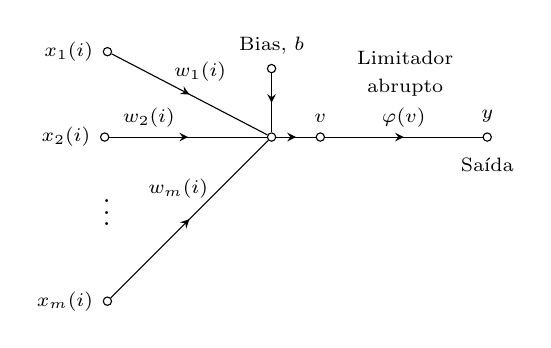
\begin{tikzpicture}[
    middlearrow/.style n args={4}{
        decoration={
            markings,
            mark=at position 0.5 with {\arrow{stealth}, \path ++(#3,#4) node[#1] {#2};}
          },
        postaction={decorate}
      },
  ]

  \node [circle,draw=black, fill=white, inner sep=0pt,minimum size=3pt,label=above:{ }] (V1) at (0, 0) {};
  \node [circle,draw=black, fill=white, inner sep=0pt,minimum size=3pt, label=left:{\scriptsize $x_1(i)$}, above left=1cm and 2cm of V1] (X1)  {};
  \node [circle,draw=black, fill=white, inner sep=0pt,minimum size=3pt, label=left:{\scriptsize $x_2(i)$}, left= 2cm of V1] (X2)  {};
  \coordinate[label={  $\vdots$}, below left=1.2cm and 2.05cm of V1] (VDOTS) {};
  \node [circle,draw=black, fill=white, inner sep=0pt,minimum size=3pt, label=left:{\scriptsize $x_m(i)$}, below left=2cm and 2cm of V1] (XM) {};
  \node [circle,draw=black, fill=white, inner sep=0pt,minimum size=3pt, label=above:{\scriptsize $v$}, right= 0.5cm of V1] (V) {};
  \node [circle,draw=black, fill=white, inner sep=0pt,minimum size=3pt, label=above:{\scriptsize $y$}, right= 2cm of V] (Y) {};

  \coordinate [ label=above:{\scriptsize Saída}, below= 0.5cm of Y] (S) {};
  
  \coordinate [ label=above:{\scriptsize Limitador}, above left= 0.75cm and 1cm  of Y] (LI) {};
  \coordinate [ label=above:{\scriptsize abrupto}, below= 0.4cm of LI] (AB) {};

  \node [circle,draw=black, fill=white, inner sep=0pt,minimum size=3pt, label=above:{ \scriptsize Bias, $b$}, above= 0.75cm of V1] (B) {};
  

  \draw [ middlearrow={above}{\scriptsize $w_1(i)$}{0.1}{0.1}] (X1) -- (V1);
  \draw [ middlearrow={above}{\scriptsize $w_2(i)$}{-0.5}{0}] (X2) -- (V1);
  \draw [ middlearrow={above}{\scriptsize $w_m(i)$}{0}{0.2}] (XM) -- (V1);
  \draw [ middlearrow={above}{ }{0}{0}] (V1) -- (V);
  \draw [ middlearrow={above}{\scriptsize $\varphi(v)$}{0}{0}] (V) -- (Y);
  \draw [ middlearrow={above}{ }{0}{0}] (B) -- (V1);

\end{tikzpicture}
\end{document}


